%\tikzset{external/export next=false}
\begin{minipage}{0.4\textwidth}
\begin{tikzpicture}
    \pgfkeys{/pgf/number format/.cd,
        fixed,
        fixed zerofill,
        precision=0,
    }

    \draw[dashed] (0,0) circle (2cm);
    \draw[dashed] (0,0) -- node[left] {$a$} (0,2);

    %\sisetup{zero-decimal-to-integer}
    \foreach \angle in {30,90,150,210,270,330} {
        \pgfmathsetmacro{\number}{\angle/60+0.5};
        \draw (\angle:2) circle (0.25cm);
        \node at (\angle:2.5) {\tiny$\pgfmathprintnumber{\number}$};
    }
\end{tikzpicture}
\end{minipage}
\begin{minipage}{0.55\textwidth}
%\tikzset{external/export next=false}
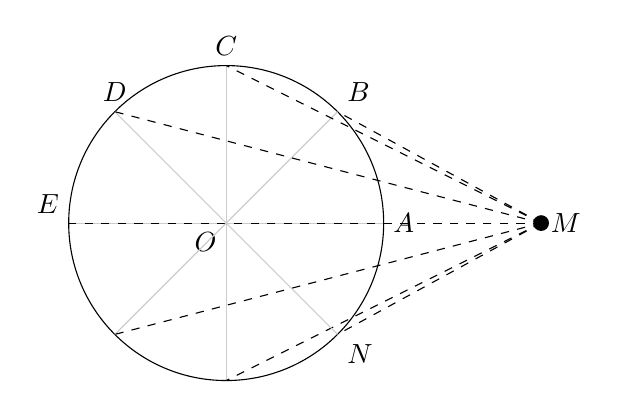
\begin{tikzpicture}
    \coordinate [label=right:$A$]       (A) at   (0:2);
    \coordinate [label=above right:$B$] (B) at  (45:2);
    \coordinate [label=above:$C$]       (C) at  (90:2);
    \coordinate [label=above:$D$]       (D) at (135:2);
    \coordinate [label=above left:$E$]  (E) at (180:2);
    \coordinate                         (F) at (225:2);
    \coordinate                         (G) at (270:2);
    \coordinate [label=below right:$N$] (N) at (315:2);
    \coordinate [label=right:$M$]       (M) at   (0:4);
    \coordinate [label=below left:$O$]  (O) at   (0,0);

    \draw (O) circle (2cm);
    \fill (M) circle (0.1cm);

    \foreach \point in {(A),(B),(C),(D),(E),(F),(G),(N)} {
        \draw[black!20] (O) -- \point;
        \draw[dashed] (M) -- \point;
    }
\end{tikzpicture}
\end{minipage}
